\section{Sicherheitsaspekte der Android-Architektur}

	Bereits durch die Architektur des Betriebssystems, insbesondere durch die restriktive Rechtevergabe und das Sandboxing, wird versucht, ein möglichst sicheres System bereitzustellen. Ab Android Version 4.3 kommt zusätzlich noch \textit{Security-Enhanced Linux (SELinux)} zum Einsatz.\\
	Verschlüsselungen und Signaturen werden Hardwareseitig durch eine \textit{Trusted Execution Environment (TEE)} unterstützt. TEE stellt einen besonders geschützten Bereich auf dem Prozessor dar, auf dem nur berechtige Anwendungen ausgeführt werden können, wie beispielsweiße die Verifikation des Bootmediums und Verschlüsselungsverfahren. Die Implementierung ist dabei Prozessor Hersteller abhängig - auf ARM wird dabei, wie bei iOS, auf \textit{TrustZone}\cite{TEE_ARM} zurückgegriffen.
	
	\subsection{Verifikation der Bootmedien} \label{sec:VerifikationDerBootmedien}
	Um bereits bei Systemstart eine Veränderung oder Ersetzung der Paritionen zu erkennen, wurde mit Android 4.4 eine Boot Verification eingeführt. Das Verfahren basiert auf der Funktion dm-verity des Device Mappers, welcher im Linux Kernel zu finden ist. Da diese Überprüfung durch den Kernel ausgeführt wird, muss vor dem Start von dm-verity erst der Bootloader und die Boot-Partition selbst auf ihre Integrität überprüft werden.
	
	\subsubsection{Integritätscheck durch den Bootloader}
	Die Verifikation des Bootloaders ist nur schwer möglich, daher wird hierbei auf eine Hardware basierende root-of-trust, hier auf Basis des TEE, gesetzt. \\
	Um die Boot- und Recovery-Parition zu validieren gibt es zwei Möglichkeiten. Für die Validierung offizieller Images wird ein in Hardware festgeschriebener, unveränderlicher, Key verwendet. Sollte dies nicht möglich sein, aufgrund eines veränderten Images, kann auf ein in der Partitionssignatur gespeichertes Zertifikat zurückgegriffen werden.
\begin{flushleft}	
	Um zu unterscheiden ob ein offizielles oder inoffizielles Image erwartet wird, kann der Bootloader zwischen zwei Status unterscheiden:\\
\end{flushleft}
	\begin{itemize}\itemsep0pt
		\item LOCKED - das aktuelle Boot-Image ist ein offizielles und kann mittels OEM Key verifiziert werden
		\item UNLOCKED - das aktuelle Boot-Image wurde verändert, und kann daher nicht mit dem OEM Key veriiziert werden
	\end{itemize}
	
\begin{flushleft}
	Diese und weitere Informationen zum Bootstatus werden in einer speziellen und besonders geschützten System Partition gespeichert. \\
\end{flushleft}
	Um eine eigene Betriebssystemversion installieren zu können, ist es zuerst notwendig, den Bootloader freizuschalten. Wurde dies getan, wird beim Hochfahren immer eine Warnung ausgegeben, um den Nutzer darauf hinzuweisen, dass die Parition nicht mittels des festgeschrieben Keys verifiziert werden konnte. Daraus ergeben sich mehrere Mögliche Zustände des Systems:\\\\
	
	\begin{figure}[h]
		\centering
		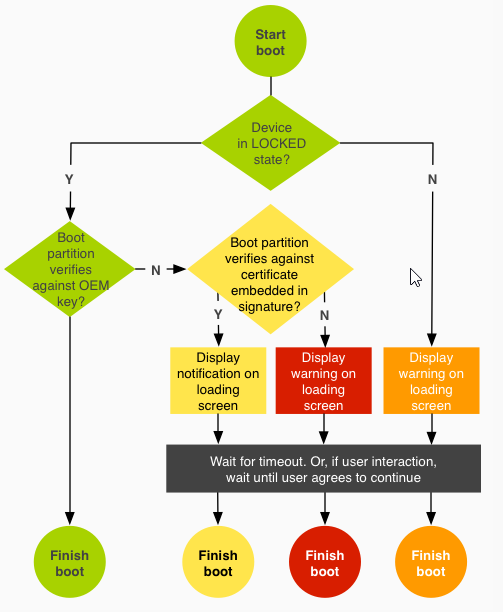
\includegraphics[width=0.7\linewidth, height=0.5\textheight]{android_pages/graphics/VerifiedBoot}
		\caption[Verified boot flow\protect\cite{VerifyingBoot}]{Verified boot flow\protect\cite{VerifyingBoot}}
		\label{fig:VerifiedBoot}
	\end{figure}
	
\begin{flushleft}
	Mit diesem Vorgehen wird auch die Integrität des Kernels sichergestellt, der das weitere Vorgehen steuert.
\end{flushleft}
	
	\subsubsection{Integritätscheck weiterer Paritionen}
	dm-verity arbeitet mit einem SHA-256 Hash-tree, der wie folgt aufgebaut ist:\\
	Für jeden 4K Sektor auf der Parition wird ein Hashwert berechnet. Jeweils zwei dieser Werte werden wiederum zu einem Neuen verrechnet. Dies wird solange wiederholt, bis nur noch ein Hashwert, der \textit{root-hash}, übrig ist. Um nun die Integrität sicherzustellen wird dieser root-hash, mit einem bereits berechneten Soll-Wert verglichen. Sind diese identisch, ist die Parition integer.
	
	\begin{figure}[h]
		\centering
		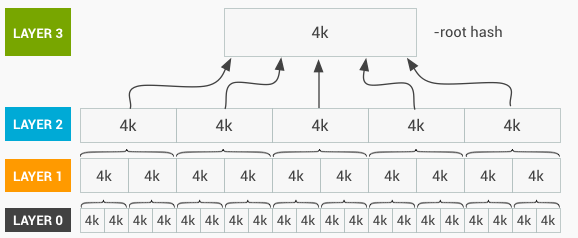
\includegraphics[width=0.7\linewidth]{android_pages/graphics/dm-verity-table}
		\caption[Aufbau des Hash-Trees]{Aufbau des von dm-verity erstellten Hash-Trees\protect\cite{VerifiedBoot}}
		\label{fig:dm-verity-table}
	\end{figure}
	
\begin{flushleft}
	Um Manipulationen am Soll-Wert zu unterbinden, wird der root-hash mit einem RSA Schlüssel signiert. Zu finden ist der Soll-Wert in der Boot-Partition.\\
\end{flushleft}
	Welche weiteren Paritionen mittels vm-verity auf ihre Integrität überprüft werden sollen, wird über einen Eintrag zu der jeweiligen Partition in der fstab-Datei festgelegt.

	\subsection{Basis Rechtesystem}\label{sec:BasisRechteSystem}
	Von Linux wurde auch das Basis-Rechtesystem Übernommen, allerdings wird es leicht abgewandelt genutzt. Anstatt das ein Nutzer des Mobilsystems eine eindeutige User-ID (UID) zugewiesen bekommt, wird jede Applikation auf dem System als ein Nutzer angesehen und bekommt zur Installationszeit eine UID. Jeder Nutzer, und somit auch jede App, arbeitet grundsätzlich erst einmal nur innerhalb der ihm zugewiesenen virtuellen Maschine und dem damit verbundenen Dateisystem.\\\\
	Da es dennoch in vielen Fällen nötig ist, Daten zwischen verschiedenen Apps auszutauschen, gibt es mehrer Möglichkeiten dies zu tun. Die üblichen Wege wären Intends oder Contentprovider. Zusätzlich gibt es noch die Möglichkeit mehreren Apps dieselbe UID zuweisen zu lassen. Dies ist allerdings nur möglich, wenn die entsprechenden Applikationen mit dem selben Zertifikat signiert wurden und in deren Manifest Datei eine gemeinsame UID festgelegt wurde.
	Durch dieses Rechtesystem wird versucht sicherzustellen, dass kein Nutzerprogramm als \textit{root} ausgeführt wird.
	
	\subsection{Sandboxing und Permissions} \label{sec:SandBoxingNPermissions}
	Wie bereits erwähnt, laufen die Applikationen jeweils in ihrer eigenen Sandbox. Grundsätzlich ist die App damit in ihrer Ausführung auf ihren Bereich beschränkt und kann nicht mit anderen Prozessen und Daten ausserhalb interagieren. Dennoch ist es in den meisten Fällen sinnvoll mit Systemservices und Nutzerdaten zu interagieren, die nicht in der eigenen Sandbox verfügbar sind. 
	
	\subsubsection{Permissions im Detail}
	Um nun die bestehenden Zugriffsrechte erweitern zu können, müssen die entsprechenden Rechte (Permissions) in der Manifest Datei deklariert und angefordert werden. Zu Installationszeit werden diese Permissions dem Nutzer angezeigt und dieser wird gefragt, ob er den Rechtswünschen der App zustimmt oder nicht. Dabei gilt das \textit{Alles-Oder-Nichts-Prinzip}, d.h. entweder bekommt die Anwendung alle Rechte oder keine - was eine nicht Installation zur Folge hat. Des weiteren können die Berechtigungen nach der Installation nicht mehr angepasst werden.\\
	Oben genannte Berechtigungen sind beispielsweiße für Zugriffe auf externe Speichermedien oder auch die Kamera nötig. Dabei ist allerdings zu beachten, dass die Permissions zum Teil sehr grob definiert sind. Wodurch für den Nutzer nicht unbedingt erkenntlich ist, welche Informationen eine App warum abgreift und ob die App wirklich Gebrauch des Rechts macht.\\
	Anhand der folgenden Permission lässt sich die daraus resultierende Problematik gut erkennen:\\
	RECORD\_AUDIO Permission:
	\begin{quote}
	Allows an application to record audio \footnote{https://developer.android.com/reference/android/Manifest.permission.html\#RECORD\_AUDIO}
	\end{quote} 
	Dabei ist für den Nutzer nicht sichtbar, wann eine Aufnahme läuft, ausser die Applikation stellt dafür einen Hinweis bereit - wobei hier die Frage ist ob dieser auch wirklich verlässlich ist. Stellt die App einen Service bereit, kann ein solcher Mitschnitt auch im Hintergrund geschehen, und damit auch während eines Telefonats. Die einzige Chance RECORD\_AUDIO zur Laufzeit zu unterbinden ist, den Service bzw. die App über den Anwendungsmanager zu beenden.\\
	Ausnahmen für diese Problematik sind Module wie GPS, WLAN und Bluetooth. Diese kann der Nutzer des Geräts abschalten und damit den Zugriff darauf verweigern.
	Dennoch ist das Problem auf viele Permissions übertragbar.\\\\
%	Für die nächste Android Version, Android M, ist eine Verbesserung dieses Berechtigungssystems geplant und auch bereits vorgestellt worden. Es wird nun ermöglicht zur Laufzeit von Applikationen diesen Berechtigungen zu entziehen und freizugeben. Damit bekommt der Nutzer deutlich mehr Möglichkeiten, um seine Daten zu schützen. Allerdings wird es wohl kein Update für ältere Versionen geben, wodurch dort das Problem bestehen bleibt.
	Mit Android 4.3 (Kitkat) wurde eine versteckte Einstellungs-Activity namens \textit{App Ops} eingeführt. Darin konnte man einsehen welche App, wann welche Permission genutzt hat, und dieser einzelne Rechte zu entziehen und wieder zu erlauben. Diese Funktion konnte nur durch das Anlegen eines Activity Shortcuts und der direkten Verwendung in einer App genutzt werden. Leider wurde diese versteckte Einstellung aus den nächsten Versionen entfernt - bis Android M. \cite{HiddenActivity} \\
	Für Android M wurde mittlerweile angekündigt, dass eine derartige Einstellung nun fest mit eingebaut sein wird.\cite{AndroidMPermission}\\
	Allerdings wird es wohl kein Update für ältere Versionen geben, wodurch das Problem in diesen bestehen bleibt.
	
	\subsubsection{Besonderheit: Systemapps}
	
	Apps der System Hersteller können Rechte besitzen, die für normale Anwendungen nicht verfügbar sind, um Basis Apps und Services bereit zustellen. Hierfür werden alle Hersteller Applikationen mit sogenannten \textit{Publisher Keys} signiert.
	
	\subsection{SELinx in Android}
	Das \textit{Discretionary Access Control (DAC)} System des Linux Kernels lässt nur relativ grobe Einstellungen zu. Hat man beispielsweiße eine Applikation, die höhere Rechte für die Ausführung benötigt, so bekommt diese unter Nutzung von DAC oftmals noch zusätzliche Rechte, welche die App nicht haben sollte.\\
	Um dieses Problem zu beheben wird seit Android 4.4 zusätzlich zum DAC noch SELinux und dessen \textit{Mandatory Access Control (MAC)} System genutzt.\\	
	\begin{quote}
	SELinux operates on the ethos of default denial. Anything that is not explicitly allowed is denied.\cite{SELinuxAndroid}
	\end{quote}
	Dabei wird, sofern das DAC System einen Zugriff gewährt, das MAC System konsultiert und nur wenn dieses auch den Zugriff gewährt. Welche Rechte eine Applikation hat und welche nicht, wird unter SELinux in MAC Policies festgehalten. 
	
	Dabei sind zwei Nutzungsmodi zu unterscheiden. Während im \textit{permissive mode} Regelverstöße nur geloggt werden, wird im \textit{enforcing mode} die strikte Einhaltung erzwungen. In den Versionen 4.3 bis exklusive 5.0 war der \textit{enforcing mode} nicht überall in Nutzung. Dies änderte sich mit Version 5.0, seit dem läuft nur noch dieser Modus.
	
	\subsection{Datenträger Verschlüsselung}
	Mit Android 3.0 (Honeycomb) wurde die Möglichkeit eingeführt, die userdata-Partition zu vollständig verschlüsseln (Fulldisk Encryption - FDE). Basis der Verschlüsselung ist, wie bei der Verifikation der Partitionen (\ref{sec:VerifikationDerBootmedien}), eine Funktion des Device Mappers - dm-crypt. %Also Verschlüsselungsalgorithmus wird 
	
	

	